\textbf{Geometry Formulas}

Triangle:

Side length $a, b, c$

Area: $\frac{1}{2} \times base \times height$

$s = \frac{a+b+c}{2}$, Area $= \sqrt{s(s-a)(s-b)(s-c)}$

Inradius: $r = \frac{Area}{s}$

Circumradius: $R = \frac{abc}{4 \times Area}$

Circles:

Arc Length: $L = \theta r$

Sector Area: $Area = \frac{1}{2} r^2 \theta$

Segment Area (Area of the part cut off by a chord): $Area = \frac{1}{2} r^2 (\theta - \sin\theta)$

\begin{itemize}
  \item \textbf{Rhombus:}
  \begin{itemize}
    \item Area: $\frac{1}{2} \times d_1 \times d_2$ (where $d_1$ and $d_2$ are diagonals).
  \end{itemize}
  \item \textbf{Trapezium:}
  \begin{itemize}
    \item Area: $\frac{1}{2} \times (\text{Base}_1 + \text{Base}_2) \times \text{Height}$.
  \end{itemize}
\end{itemize}
3. \textbf{Regular Polygon} (\textit{n sides}):
\begin{itemize}
  \item Perimeter: $n \times a$
  \item Area: $\frac{1}{4}na^2 \cot\!\left(\frac{\pi}{n}\right)$ (where $a$ is the side length).
\end{itemize}

\textbf{Curved Shapes}

1. \textbf{Circle}
\begin{itemize}
  \item Circumference: $2\pi r$
  \item Area: $\pi r^2$
\end{itemize}
2. \textbf{Ellipse}
\begin{itemize}
  \item Area: $\pi a b$ (where $a$ is the semi-major axis and $b$ is the semi-minor axis).
\end{itemize}

\textbf{$\checkmark$ Polygon}

\begin{itemize}
  \item Interior angle sum:
  $(n-2) \times 180^{\circ}$

  \item Each internal angle (regular):
  $\frac{(n-2)\times180^{\circ}}{n}$
\end{itemize}

4. \textbf{Tetrahedron}
\begin{itemize}
  \item Volume: $\frac{1}{6} \times \text{Base Area} \times \text{Height}$.
\end{itemize}

\textbf{Curved 3D Shapes}

1. \textbf{Sphere}
\begin{itemize}
  \item Surface Area: $4\pi r^2$
  \item Volume: $\frac{4}{3}\pi r^3$
\end{itemize}
2. \textbf{Cylinder}
\begin{itemize}
  \item Surface Area: $2\pi r(r+h)$
  \item Volume: $\pi r^2 h$
\end{itemize}
3. \textbf{Cone}
\begin{itemize}
  \item Surface Area: $\pi r(r+l)$, where $l=\sqrt{r^2+h^2}$ is the slant height.
  \item Volume: $\frac{1}{3}\pi r^2 h$.
\end{itemize}

\textbf{Other Shapes}

1. \textbf{Torus}
\begin{itemize}
  \item Surface Area: $4\pi^2 Rr$
  \item Volume: $2\pi^2 Rr^2$, where $R$ is the distance from the center of the tube to the center of the torus, and $r$ is the radius of the tube.
\end{itemize}

\vspace{2em}
\begin{center}
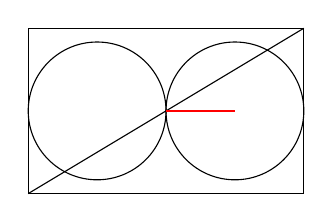
\begin{tikzpicture}[scale=0.7]
  \draw (0,0) rectangle (5,3);
  \draw (1.25,1.5) circle (1.25);
  \draw (3.75,1.5) circle (1.25);
  \draw (0,0) -- (5,3);
  \draw[red, thick] (2.5,1.5) -- (3.75,1.5);
\end{tikzpicture}
\end{center}
\vspace{1em}

\vspace{2em}
\begin{center}
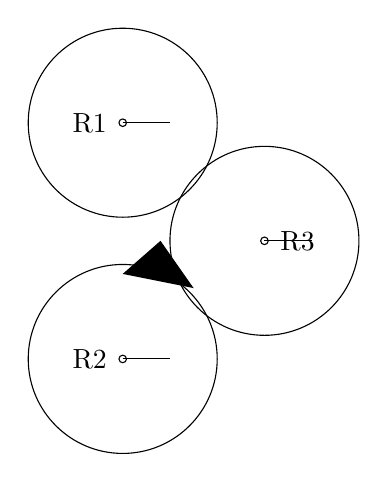
\begin{tikzpicture}[scale=0.6]
  \draw (0,2.5) circle (2);
  \draw (3,0) circle (2);
  \draw (0,-2.5) circle (2);
  \fill[black] (0.8,0) -- (0,-0.7) -- (1.5,-1) -- cycle;
  \draw (0,2.5) circle (0.08);
  \draw (3,0) circle (0.08);
  \draw (0,-2.5) circle (0.08);
  \node at (-0.7,2.5) {R1};
  \node at (3.7,0) {R3};
  \node at (-0.7,-2.5) {R2};
  \draw (0,2.5) -- ++(1,0);
  \draw (3,0) -- ++(1,0);
  \draw (0,-2.5) -- ++(1,0);
\end{tikzpicture}
\end{center}
